\documentclass[crop,tikz,convert={outext=.svg,command=\unexpanded{pdf2svg \infile\space\outfile}}]{standalone}

\usepackage{tikz}
\usetikzlibrary{backgrounds}

\begin{document}

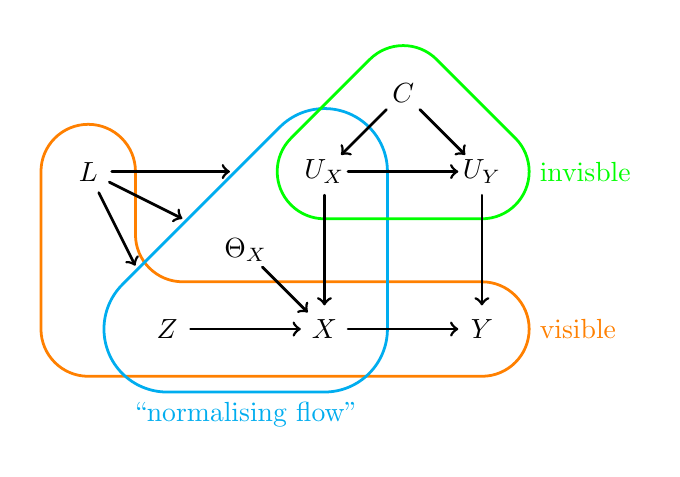
\begin{tikzpicture}[
  line cap=round,
  line join=round,
  line width=1pt,
  x=2cm,
  y=2cm,
  show background rectangle,
  background rectangle/.style={
    fill=white,
    draw=none,
  },
]

  \draw[orange] (-0.2,1) arc(0:180:0.3) -- (-0.8,0) arc(180:270:0.3) -- (2,-0.3) arc (-90:90:0.3) -- (0.1,0.3) arc(270:180:0.3) -- cycle;
  \node[orange,anchor=west] at (2.3,0) {visible};

  \draw[cyan] (0,-0.4) -- (1,-0.4) arc (-90:0:0.4) -- (1.4,1) arc(0:135:0.4) -- ({-0.4/sqrt(2)},{0.4/sqrt(2)}) arc (135:270:0.4) -- cycle;
  \node[cyan,anchor=north] at (0.5,-0.4) {``normalising flow"};

  \draw[green] (1,0.7) -- (2,0.7) arc (-90:45:0.3) -- ({1.5+0.3/sqrt(2)},{1.5+0.3/sqrt(2)}) arc(45:135:0.3) -- ({1-0.3/sqrt(2)},{1+0.3/sqrt(2)}) arc (135:270:0.3) -- cycle;
  \node[green,anchor=west] at (2.3,1) {invisble};

  \node at (0,0) {$Z$};
  \node at (-0.5,1) {$L$};
  \node at (1,0) {$X$};
  \node at (2,0) {$Y$};
  \node at (1,1) {$U_X$};
  \node at (2,1) {$U_Y$};
  \node at (1.5,1.5) {$C$};
  \node at (0.5,0.5) {$\Theta_X$};
  \draw[->, shorten <=3mm, shorten >=3mm] (0,0) -- (1,0);
  \draw[->, shorten <=3mm, shorten >=3mm] (1,0) -- (2,0);
  \draw[->, shorten <=3mm, shorten >=3mm] (1,1) -- (2,1);
  \draw[->, shorten <=3mm, shorten >=3mm] (1,1) -- (1,0);
  \draw[->, shorten <=3mm, shorten >=3mm] (2,1) -- (2,0);
  \draw[->, shorten <=3mm, shorten >=3mm] (1.5,1.5) -- (1,1);
  \draw[->, shorten <=3mm, shorten >=3mm] (1.5,1.5) -- (2,1);
  \draw[->, shorten <=3mm, shorten >=3mm] (0.5,0.5) -- (1,0);
  \draw[->, shorten <=3mm, shorten >=9mm] (-0.5,1) -- (0,0);
  \draw[->, shorten <=3mm, shorten >=9mm] (-0.5,1) -- (0.5,0.5);
  \draw[->, shorten <=3mm, shorten >=12mm] (-0.5,1) -- (1,1);

\end{tikzpicture}
\end{document}
